%% History:
% Pavel Tvrdik (26.12.2004)
%  + initial version for PhD Report
%
% Daniel Sykora (27.01.2005)
%
% Michal Valenta (3.12.2008)
% rada zmen ve formatovani (diky M. Duškovi, J. Holubovi a J. Žďárkovi)
% sjednoceni zdrojoveho kodu pro anglickou, ceskou, bakalarskou a diplomovou praci

% One-page layout: (proof-)reading on display
%%%% \documentclass[11pt,oneside,a4paper]{book}
% Two-page layout: final printing
\documentclass[11pt,twoside,a4paper]{book}
%=-=-=-=-=-=-=-=-=-=-=-=--=%
% The user of this template may find useful to have an alternative to these
% officially suggested packages:
\usepackage[czech, english]{babel}

\usepackage[T1]{fontenc} % pouzije EC fonty
% pripadne pisete-li cesky, pak lze zkusit take:
% \usepackage[OT1]{fontenc}
\usepackage[utf8]{inputenc}

\usepackage{tikz}
\usepackage{amsmath}
\usepackage{listings}
%=-=-=-=-=-=-=-=-=-=-=-=--=%
% In case of problems with PDF fonts, one may try to uncomment this line:
%\usepackage{lmodern}
%=-=-=-=-=-=-=-=-=-=-=-=--=%
%=-=-=-=-=-=-=-=-=-=-=-=--=%
% Depending on your particular TeX distribution and version of conversion tools
% (dvips/dvipdf/ps2pdf), some (advanced | desperate) users may prefer to use
% different settings.
% Please uncomment the following style and use your CSLaTeX (cslatex/pdfcslatex)
% to process your work. Note however, this file is in UTF-8 and a conversion to
% your native encoding may be required. Some settings below depend on babel
% macros and should also be modified. See \selectlanguage \iflanguage.
%\usepackage{czech}  %%%%%\usepackage[T1]{czech} %%%%[IL2] [T1] [OT1]
%=-=-=-=-=-=-=-=-=-=-=-=--=%

%%%%%%%%%%%%%%%%%%%%%%%%%%%%%%%%%%%%%%%
% Styles required in your work follow %
%%%%%%%%%%%%%%%%%%%%%%%%%%%%%%%%%%%%%%%
\usepackage{graphicx}

%%1. odstavec jako v cestine.
%\usepackage{indentfirst}

% thesis formatting macros
\usepackage{k336_thesis_macros}

% work type
\newcommand\TypeOfWork{Diplomová práce} \typeout{Diplomova prace}

% study program
\newcommand\StudProgram{Otevřená informatika, Navazující magisterský}

% study branch
\newcommand\StudBranch{Softwarové inženýrství}

%
% Work title, author, etc.
%
\newcommand\WorkTitle{Validace principů objektového návrhu v kódu}
\newcommand\FirstandFamilyName{Bc. Martin Vejmelka}
\newcommand\Supervisor{Ing. Ondřej Macek}

% Pouzijete-li pdflatex, tak je prijemne, kdyz bude mit vase prace
% funkcni odkazy i v pdf formatu
\usepackage[
  pdftitle={\WorkTitle},
  pdfauthor={\FirstandFamilyName},
  bookmarks=true,
  colorlinks=true,
  breaklinks=true,
  urlcolor=red,
  citecolor=blue,
  linkcolor=blue,
  unicode=true,
]{hyperref}

% Extension posted by Petr Dlouhy in order for better sources reference (\cite{} command) especially in Czech.
% April 2010
% See comment over \thebibliography command for details.

\usepackage[square, numbers]{natbib}             % sazba pouzite literatury
%\usepackage{url}
%\DeclareUrlCommand\url{\def\UrlLeft{<}\def\UrlRight{>}\urlstyle{tt}}  %rm/sf/tt
%\renewcommand{\emph}[1]{\textsl{#1}}    % melo by byt kurziva nebo sklonene,
\let\oldUrl\url
\renewcommand\url[1]{<\texttt{\oldUrl{#1}}>}

\usepackage{nameref}

\begin{document}

\selectlanguage{czech}

\iflanguage{czech}{
  \typeout{************************************************}
  \typeout{Zvoleny jazyk: cestina}
  \typeout{Typ prace: \TypeOfWork}
  \typeout{Studijni program: \StudProgram}
  \typeout{Obor: \StudBranch}
  \typeout{Jmeno: \FirstandFamilyName}
  \typeout{Nazev prace: \WorkTitle}
  \typeout{Vedouci prace: \Supervisor}
  \typeout{***************************************************}
  \newcommand\Department{Katedra počítačové grafiky a interakce}
  \newcommand\Faculty{Fakulta elektrotechnická}
  \newcommand\University{České vysoké učení technické v Praze}
  \newcommand\labelSupervisor{Vedoucí práce}
  \newcommand\labelStudProgram{Studijní program}
  \newcommand\labelStudBranch{Obor}
}{
  \typeout{************************************************}
  \typeout{Language: english}
  \typeout{Type of Work: \TypeOfWork}
  \typeout{Study Program: \StudProgram}
  \typeout{Study Branch: \StudBranch}
  \typeout{Author: \FirstandFamilyName}
  \typeout{Title: \WorkTitle}
  \typeout{Supervisor: \Supervisor}
  \typeout{***************************************************}
  \newcommand\Department{Department of Computer Science and Engineering}
  \newcommand\Faculty{Faculty of Electrical Engineering}
  \newcommand\University{Czech Technical University in Prague}
  \newcommand\labelSupervisor{Supervisor}
  \newcommand\labelStudProgram{Study Programme}
  \newcommand\labelStudBranch{Field of Study}
}

%
% Title page
%
\coverpagestarts

%
% Acknowledgements
%
\acknowledgements
\noindent
TODO: Zde můžete napsat své poděkování, pokud chcete a máte komu děkovat.

%
% Declaration
%
% TODO: supply valid date
\declaration{V~Praze dne 15.\,5.\,2008}

%
% Abstract
%
\abstractpage

% TODO: Translation of Czech abstract into English.

% Prace v cestine musi krome abstraktu v anglictine obsahovat i
% abstrakt v cestine.
\vglue60mm

\noindent{\Huge \textbf{Abstrakt}}
\vskip 2.75\baselineskip

\noindent
TODO: Abstrakt práce by měl velmi stručně vystihovat její podstatu. Tedy čím se práce zabývá a co je jejím výsledkem/přínosem.

\noindent
Očekávají se cca 1 -- 2 odstavce, maximálně půl stránky.

%
% Table of Contents
%
\tableofcontents

%
% List of Figures
%
\listoffigures

%
% List of Tables
%
\listoftables

%
% Initial settings and start of real work text
%

\mainbodystarts
% horizontalní mezera mezi dvema odstavci
%\parskip=5pt
%11.12.2008 parskip + tolerance
\normalfont
\parskip=0.2\baselineskip plus 0.2\baselineskip minus 0.1\baselineskip

%
% Chapters
%

\chapter{Úvod}

\section{Motivace projektu, záměr práce}
\label{introduction-motivation}

Při realizaci softwarových projektů zpravidla postupujeme od sběru požadavků, přes \emph{analýzu} a \emph{návrh} až k~\emph{fyzické realizaci} programového produktu ve zdrojovém kódu vhodného programovacího jazyka \cite{wiki:sdlc}. Vytvořením reprezentace systému ve zdrojovém kódu však životní cyklus softwarového díla nekončí. Vedle \emph{testování}, \emph{integrace}, \emph{akceptace} a \emph{dodávky} je nutné ještě uvažovat o~další fázi -- \emph{údržbě}. Pro tyto fáze, které jsou neméně důležité, leč mnohdy opomíjené, je kritická především \emph{architektura systému}.

Architektura existujícího systému je většinou definována poměrně vágně. Při dalších úpravách se tak můžeme spolehnout na malou podmnožinu pravidel, kterou u~daného systému předpokládáme a která často ani nemusí platit. Vždy se však můžeme spolehnout na to, že pokud zdrojový kód programového produktu projde bez chyb překladačem nebo interpretrem programovacího/skriptovacího jazyka, v~němž je napsán, jedná se o~kód podléhající pravidlům tohoto jazyka.

Syntaxe jazyka je definována gramatikou, sémantika potom dává jednotlivým konstruktům jazyka jejich význam (např. \verb+for+ bude znamenat opakované provádění kódu mezi počáteční \verb+{+ a koncovou \verb+}+ složenou závorkou následujícího bloku).

Kromě struktury, kterou vynucuje překladač jazyka bývá často zavedena množina kódových konvencí. Vedle konvencí pro formátování zdrojového kódu (které nemají z~hlediska analýzy architektury systému význam) můžeme zmínit konvence, které zakazují aby měla metoda více než nějaký daný počet příkazů/parametrů, konvence, které nařizují, aby se v~kódu nevyskytovaly neprovolávané (mrtvé) části kódu, a další.

V~této práci se pokusíme zmíněné konvence zachytit jako pravidla, která lze vhodným způsobem ověřit. Znázornění tohoto konceptu je na obrázku \ref{work_scope}.
\begin{figure}[h!]
  \centering
  \begin{tikzpicture}
    \shadedraw  (0,0) rectangle (4,4);
    \shadedraw  (4.2,0) rectangle (8.2,4);
    \draw  (0,4.2) rectangle (4.0,8.2);
    \draw  (4.2,4.2) rectangle (8.2,8.2);

    \draw  (2,2) node[text width=2.5cm, text centered] {množina pravidel};
    \draw  (6.2,2) node[text width=2.5cm, text centered] {instance splňující pravidla};
    \draw  (2,6.2) node[text width=2.5cm, text centered] {gramatika a standardní knihovny};
    \draw  (6.2,6.2) node[text width=2.5cm, text centered] {instance jazyka generovaného gramatikou};

    \draw (-2,2) node[text width=2.5cm, text centered] {kódové konvence (těžko vynutitelné)};
    \draw (-2,6.2) node[text width=2.5cm, text centered] {definice programovacího jazyka};

    \draw (2,8.6) node[text width=2.5cm, text centered] {meta-model};
    \draw (6.2,8.6) node[text width=2.5cm, text centered] {model};
  \end{tikzpicture}
  \caption{Rozšíření gramatiky jazyka o~množinu pravidel.\label{work_scope}}
\end{figure}
Množina pravidel zpřesní meta-model tvořený gramatikou jazyka -- omezí množiny instancí daného jazyka na podmnožinu, která splňuje požadovaná pravidla.

Jistou analogii můžeme vidět ve značkovacím jazyku XML v~pojmech \emph{well-formedness} versus \emph{validity}. Gramatika udává, že se v~textu mohou vyskytovat elementy a atributy, že se nesmí \uv{křížit} jednotlivé tagy atd. Další dodatečná informace (DTD, XSchema, RELAX NG, atd.) potom zpřesní, jaké tagy, v~jakém pořadí a počtu se smí ve výsledné instanci XML dokumentu vyskytovat.

\section{Úvod do řešené problematiky}

Architektura softwarového systému \cite{wiki:software_architecture} je dána množinou pravidel a tvrzení o~uspořádání systému, která platí pro daný softwarový systém. Architekturu zpravidla uvažujeme z~různých pohledů (views) \cite{wiki:four_plus_one_views}, které popisují systémové komponenty a vztahy mezi nimi vždy z~úhlu některé ze zainteresovaných stran (stakeholders). Např. \emph{logical view} se zabývá architekturou z~pohledu funkcionality, kterou systém poskytuje \emph{koncovým uživatelům}, \emph{physical view} poskytuje pohled pro \emph{systémového inženýra} -- uspořádání komponent v~systému a propojení mezi nimi.

Pro systémového návrháře bude nejdůležitější právě architektura na fyzické úrovni, se kterou bude muset dále pracovat v~případě dodatečných zásahů do systému. Jedná se o~vztahy mezi konkrétními komponentami realizované v~existujícím systému. Ačkoliv sem spadají všechny komponenty systému (tedy i hardwarové), budeme se v~této práci zabývat zejména jeho softwarovými součástmi -- funkčními bloky a moduly.

Základní prostředky pro dělení softwarového díla na vhodné funkční moduly a bloky poskytuje již většina moderních programovacích jazyků. Různé programovací jazyky podporují různá paradigmata a následně i strukturování zdrojových kódů programu \cite{wiki:programming_paradigm}. Ve funkcionálním programovacím jazyku budeme strukturovat dílo do zanořených funkcí, u~objektově orientovaného programování budou základními moduly třídy a balíčky. V~textu práce se zaměříme právě na objektově orientované programovací jazyky.

Prostředky jazyka, které podporují správný návrh software rozšíříme navíc o~množinu pravidel tak, jak bylo uvedeno v~sekci \ref{introduction-motivation}. Množina těchto pravidel může být formulována neformálně ve formě požadavků na to, co by měla splňovat výsledná architektura. Uveďme příklady takových formulací:

\begin{itemize}
\item \uv{v~běžném kódu by se neměla vyskytovat (nestatická) pole s~modifikátorem \emph{public}, pouze \emph{private}, k~nimž se přistupuje pomocí \emph{getterů} a \emph{setterů}},
\item \uv{třídy z~balíčku A~nesmí záviset na jiných nesystémových \emph{třídách}, ale nejvýše na \emph{rozhraních} balíčku B} (programování proti rozhraní namísto proti konkrétní implementaci),
\item \uv{třídy v~tomto balíčku smí mít maximálně pět metod, z~nichž každá smí mít nejvýše tři parametry} (může být konvence v~nějaké firmě),
\end{itemize}

Podobné neformální specifikace se pokusíme přeformulovat pomocí vhodně zvoleného formalismu do pravidel, která bude možné následně vyhodnotit a na základě výstupu buď navrhnout nebo (je-li to možné) opravit návrh tak, aby pravidla splňoval.

\section{Struktura práce}

Práce je strukturována na základě běžného životního cyklu softwarového projektu. \emph{Úvodní kapitola} zahrnuje motivaci a deklaraci záměru práce a poskytuje úvod do řešené problematiky. V kapitole druhé (\emph{specifikace cílů práce}) jsou specifikovány konkrétní požadavky na výsledky práce. Fáze \emph{analýzy} (kapitola \ref{analysis}) postupně provádí rešerši problematiky správného návrhu software, zabývá se analýzou projektů, které budou vstupem pro vyvíjený nástroj a poskytuje přehled o existujících možnostech zpracování zdrojového kódu v jazyce Java. \emph{Návrh} řešení je poskytován v kapitole \ref{design}. Zde se zabýváme jednak návrhem formalizace pravidel pomocí vhodné matematické reprezentace a dále návrhem samotného nástroje pro ověřování těchto pravidel. Popis implementace návrhu je poskytován v kapitole \ref{implementation}. V této kapitole se zaměřujeme na podstatné části implementace. Je zde provedena formalizace pravidla \emph{Law of Demeter} pomocí navrženého formalismu. Taktéž jsou na tomto místě popsány zajímavé implementační detaily vyvíjeného systému. Kapitola \emph{testování} popisuje prováděné testování systému. \emph{Závěr} shrnuje obsah a výsledky práce.

V přílohách nalezne čtenář seznam zkratek použitých v textu této práce, instalační a uživatelskou příručku realizovaného systému a popis obsahu přiloženého CD, které je nedílnou součástí této práce.

\chapter{Specifikace cílů práce}

Účelem této sekce je stanovení přesného popisu řešené problematiky a cílů práce. Tyto cíle popíšeme formou požadavků na výsledky práce. Při specifikaci požadavků budeme vycházet ze zadání. Na základě zadání můžeme specifikovat tři oblasti požadavků.

V~první oblasti se budeme zabývat požadavky na rešeršní části práce -- analýzu \emph{principů} používaných při \emph{objektově orientovaném návrhu a implementaci}. Část druhá bude obsahovat požadavky na \emph{formalizaci pravidel}, která umožní popsat principy analyzované v~části první. Třetí část poskytne rozbor \emph{požadavků na systém}, který by měl demonstrovat vyhodnocování/validaci definovaných pravidel na existujících zdrojových kódech.

Na konci kapitoly rozebereme v~rámci jedné sekce existující podobná řešení/nástroje, jejich výhody a nevýhody.

\section{Požadavky na analýzu základních návrhových principů}
\label{requirements-principle_analysis}
Zadání práce specifikuje konkrétně tři návrhové principy -- \emph{low coupling}, \emph{high cohesion} a \emph{Law of Demeter}. Tyto principy jsou si v~mnohém podobné. Všechny se zabývají zejména závislostmi mezi částmi zdrojových kódů a jejich propojeností.

V~části analýzy je nutné projít postupně tyto návrhové principy a určit jejich vlastnosti a možnosti ověřování. To zahrnuje zejména provedení rešerší a specifikaci konkrétních tvrzení, která bude následně možné převést na pravidla. Může se ukázat, že ne všechny principy jsou exaktně definované, ověřitelné a vynutitelné. V~takových případech je možné uvažovat spíše statistický přístup oproti ověřování pravidel. Výsledkem by potom nebyl výsledek splňuje/nesplňuje, ale např. množina statistických atributů (features), na níž by bylo možné provádět další druhy analýzy (klasifikaci, pattern matching, \ldots).

Výsledkem analýzy principů by mělo být především vymezení oblasti, kterou se budeme zabývat v~další části -- \emph{formalizaci pravidel}.

\section{Požadavky na formalizaci pravidel}

Formalizace pravidel bude mít dvě hlavní součásti. V~obecné části bude definován model nad nímž budeme stavět pravidla a formát/způsob zápisu pravidel. Konkrétní část potom poskytne specifikaci pravidel \emph{Law of Demeter}, \emph{low coupling} a \emph{high cohesion} v~navrženém formalismu (bude-li to možné).

Definice modelu bude zahrnovat určení vhodné reprezentace problémové domény. Je třeba provést namapování analyzovaných objektů (elementy zdrojového kódu) na zvolenou reprezentaci domény (model) a poskytnout jazyk, pomocí něhož bude možné specifikovat pravidla, která chceme ověřit.

Po vytvoření vhodného modelu je nutné tento model následně převést do počítačové reprezentace a poskytnout vhodnou serializaci navrženého jazyka\footnote{Jazyk může obsahovat různé matematické symboly ($\forall$, $\exists$, atd.), které je obtížné zadávat do počítače přímo. Proto je vhodné poskytnout alternativní reprezentaci jazyka zahrnující pouze omezené množství znaků.}, abychom mohli pravidla vyhodnotit pomocí systému pro vyhodnocování pravidel.

\section{Požadavky na systém pro vyhodnocování pravidel}
\label{requirements-rules_evaluation}
Třetí část požadovaná zadáním zahrnuje vytvoření nástroje pro ověřování pravidel. Vstupem pro tento nástroj bude \emph{množina pravidel} a vhodně předzpracované zdrojové kódy analyzovaného projektu (\emph{vstupní projekt}). Nástroj může být navržen obecněji, budeme-li na vstupu předpokládat vhodnou vnitřní reprezentaci zdrojových kódů. Doprogramováním vstupních modulů\footnote{Vstupní moduly musí provést zparsování zdrojových kódu, vygenerování AST a rozlišení jmen a typů (name/type resolution).} bude možné poskytnout podporu i pro další jazyky.

Celková struktura výsledného projektu je znázorněna na obrázku \ref{requirements-system_structure}.

\begin{figure}[h!]
  \centering
  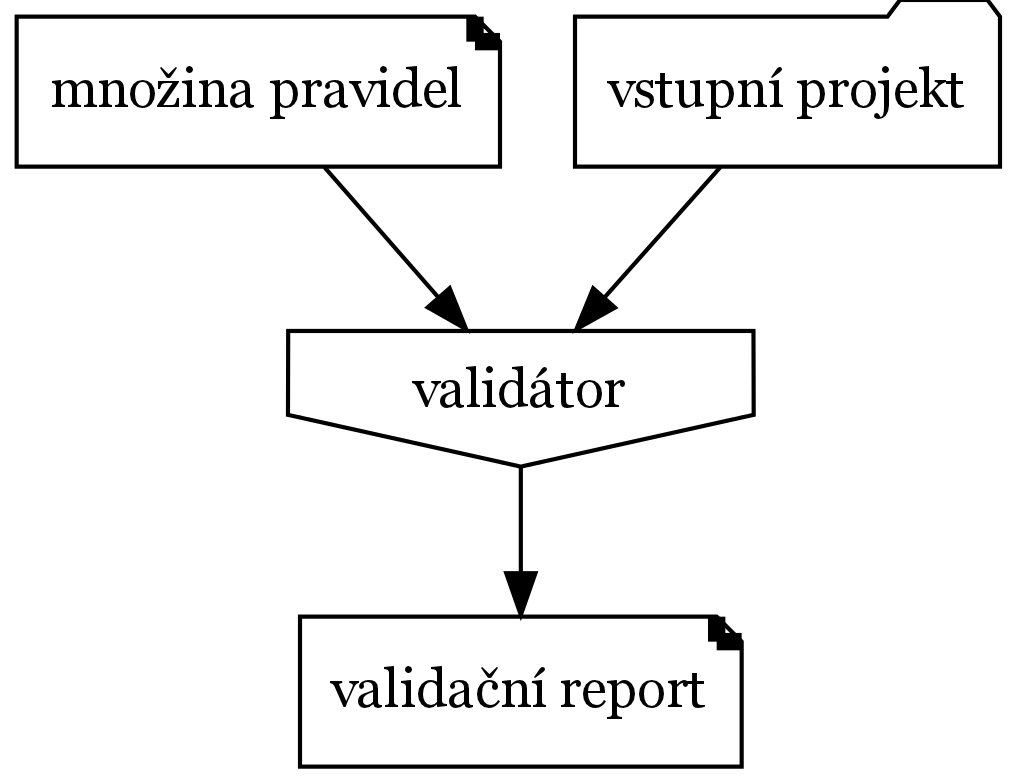
\includegraphics[width=0.5\textwidth]{./graphs/global_structure.png}
  \caption{Struktura systému.\label{requirements-system_structure}}
\end{figure}

Výstupem systému by měl být \emph{validační report}, který vypíše, která pravidla ze vstupního souboru byla porušena. Formát vstupních pravidel a výstupního reportu bude definován dále.

\subsection{Funkční požadavky na výsledný systém}

Na základě obecných požadavků můžeme specifikovat základní funkční požadavky. Požadujeme, aby systém uměl provádět následující funkčnosti:
\begin{itemize}
\item načíst vhodně předzpracovaný projekt realizovaný v jazyce Java a vytvořit vnitřní model pro další analýzu,
\item načíst ze vstupního souboru množinu pravidel v~definovaném formátu,
\item provést validaci načteného modelu pomocí množiny pravidel,
\item vypsat report obsahující informace o~splnění resp. porušení pravidel.
\end{itemize}

\subsection{Nefunkční požadavky na výsledný systém}
Z~nefunkční požadavků je zadáním práce dán požadavek na \emph{rozšiřitelnost}. Systém by mělo být možné rozšířit o~další modely a možnosti specifikace nových/složitějších pravidel nad modely.

\section{Rešerše existujících řešení}
\label{requirements-existing_tools}

V~této sekci se postupně podíváme na různé nástroje, které si kladou za cíl ověřování kvality kódu na různých úrovních. Každý z~těchto nástrojů pojímá kontrolu kvality zdrojového kódu poněkud jiným způsobem. Některé se zabývají \uv{pouhou} analýzou na úrovni jedné kompilační jednotky\footnote{Kompilační jednotka je u~jazyka Java představována jedním \verb-*.java- souborem.}, jiné provádějí strukturální analýzu na úrovni vztahů mezi jednotlivými třídami.

\subsection{CheckStyle}
\emph{CheckStyle} je vývojový nástroj, který si klade za cíl pomoci programátorům psát Java kód, který vyhovuje konkrétním kódovým konvencím \cite{existingtools:checkstyle}. Pracuje na úrovni jednoduchého zpracovávání \verb+*.java+ souborů a kontroluje např. přítomnost \verb+javadoc+ komentářů nad třídami, atributy a metodami, jmenné konvence, maximální povolené počty parametrů, délky řádků, duplicitní kód atd. \cite{existingtools:checkstyle-wiki}. Zvládne i jednodušší testy na zjištění složitosti kódu (podle klíčových slov for, while, atd.). Kódové konvence jsou konfigurovatelné pomocí XML souborů, kde lze vybírat, která předdefinovaná pravidla se budou v~kódu kontrolovat (např. pravidlo \mbox{\uv{AvoidStarImport}} apod.).

\subsection{DP-Miner}
Autoři článku \cite{4273268} a nástroje \emph{DP-Miner} \cite{existingtools:dp-miner} se zabývají výzkumem v~oblasti návrhových vzorů. Ukazuje se, že návrhové vzory jsou velmi důležité a extenzivně využívané ve fázi návrhu software. Při realizaci v~konkrétním zdrojovém kódu se však informace o~návrhových vzorech zpravidla ztrácí. Cílem nástroje \emph{DP-Miner} je objevování návrhových vzorů v~existujících projektech, k~nimž neexistuje vývojová dokumentace. Ve článku \cite{4273268} jsou demonstrovány schopnosti odhalit návrhové vzory na reálných projektech jako např. \emph{JUnit}, \emph{JEdit}, \emph{Java.AWT} a dalších. Pro odhalování vzorů používají autoři matici vztahů mezi třídami analyzovaného systému.

\subsection{FindBugs}
Nástroj \emph{FindBugs} \cite{existingtools:findbugs} vyhledává potenciální zdroje chyb v~Java programech. Vyhledává chyby podle chybových vzorů. Chybové zdroje jsou idiomy, které se ve zdrojových kódech často vyskytují chybně použity. Většinou se jedná o~obtížněji zvládnutelné vlastnosti jazyka, nepochopení rozhraní některého API atd. (Typickým příkladem může být porovnávání objektů \verb+String+ pomocí operátoru \verb+==+.) Pro odhalování chyb je používána statická analýza. \emph{FindBugs} pracuje nad byte kódem (analyzuje zkompilované třídní \verb-*.class- soubory) -- \mbox{je tedy} možné analyzovat i programy, k~nimž nemáme k~dispozici zdrojové kódy. Analýza je mnohdy nepřesná (ne všechny vzory chyb jsou vždy opravdu chybami -- může se jednat o~záměrné použití). Nástroj v~takovém případě chybně vypisuje varování, která neznamenají chybu (falešně pozitivní případy).

\subsection{JDepend}
Podobně jako předchozí nástroj pracuje i \emph{JDepend} \cite{existingtools:jdepend} nad zkompilovanými \verb+*.class+ soubory jazyka Java. Funguje však na jiném principu a na daleko vyšší úrovni. Zabývá se analýzou závislostí mezi třídami a balíčky. Systém poskytuje výpis základních metrik, jako je počet tříd a rozhraní v~balíčcích, počet závislých balíčků (to je zde označováno jako \uv{zodpovědnost} -- čím více tříd na balíčku závisí, tím větší je jeho zodpovědnost). Vesměs se jedná o~metriky založené na počtech elementů v~projektu. Za zmínku stojí odhalování cyklů v~závislostech balíčků.

\subsection{Macker}
Velmi zajímavým nástrojem je \emph{Macker} \cite{existingtools:macker}. Pracuje na strukturální úrovni během kompilace a umožňuje kontrolovat nejrůznější strukturální pravidla. Stejně jako předchozí dva nástroje operuje nad zkompilovanými \verb+*.class+ soubory. Mezi zajímavá pravidla, která je schopen vynutit patří například:

\begin{itemize}
\item \uv{třídy z~UI vrstvy nesmí přímo přistupovat k~objektům v~datové vrstvě nebo používat třídy v~balíčku \verb-java.sql-},
\item \uv{externí systémy nesmí přistupovat k~interním implementačním třídám (které mají sufix 'Impl')},
\item \uv{jeden funkční modul smí přistupovat ke druhému pouze přes jeho API}.
\end{itemize}

Z~uvedených pravidel je patrné, že \emph{Macker} operuje na globální strukturální úrovni a je schopen vynutit dodatečnou kontrolu přístupu (vedle standardních prostředků jazyka Java, kterými jsou modifikátory přístupu).

\subsection{PMD}
Velmi rozšířený nástroj \emph{PMD} \cite{existingtools:pmd} prochází zdrojové kódy jazyka Java a vyhledává potenciální zdroje problémů (srov. s~nástrojem \emph{FindBugs}). Příkladem vyhledávaných vzorů jsou:

\begin{itemize}
\item možné chyby -- prázdné příkazy \emph{try/catch/finally/switch},
\item mrtvý kód -- nepoužité lokální proměnné, parametry a privátní metody\footnote{To je dnes běžné téměř pro všechna nejčastěji používaná IDE pro vývoj v~jazyce Java.},
\item neoptimální kód -- neefektivní využívání tříd String/StringBuffer,
\item příliš komplikované výrazy -- zbytečné \verb+if+ příkazy, cykly \verb+for+, které mohou být realizovány pomocí \verb+while+.
\end{itemize}

Výhodou \emph{PMD} je integrovanost s~velkým množstvím nástrojů (JDeveloper, Eclipse, JEdit, JBuilder, ItelliJ IDEA, Maven, Emacs, a další).

\subsection{QJ-Pro}
Dalším pokročilým nástrojem je \emph{QJ-Pro} \cite{existingtools:qjpro}. Pracuje nad zdrojovými kódy a poskytuje velké množství pravidel, která lze vyhodnocovat. Kromě vynucení běžných kódových konvencí podporuje navíc analýzu nejrůznějších metrik (počet metod na třídu, poměr privátních a public polí, a další.). Existuje integrace do vývojových prostředí -- např. Eclipse IDE a~Borland JBuilder.

\subsection{Soot}
Poněkud odlišným nástrojem je \emph{Soot} \cite{existingtools:soot}. Jedná se o~framework pro optimalizaci Java kódu. Na rozdíl od předchozích zmiňovaných nástrojů, které jsou určeny spíše běžným programátorům, se jedná výzkumný projekt a platformu, na které je možné vyvíjet nástroje pro optimalizaci a analýzu. Nástroj pracuje nad Java byte kódem. Existuje integrace do Eclipse IDE.

\subsection{Squale}
\emph{Squale}\footnote{Uvedený název je odvozen z~úplného názvu \uv{Software QUALity Enhancement}.} \cite{existingtools:squale} je opět zcela jiný pohled na práci se zdrojovými kódy. Nejedná se o~běžný analyzátor kódu (jako téměř všechny předchozí případy) ale spíše o~monitorovací nástroj, který umožní sledovat přehledně metriky zdrojových kódů. Případy užití tohoto nástroje tedy spadají spíše do oblasti managementu (vyhodnocování výkonnosti týmu, kvality jejich kódu atd.).

\chapter{Analýza}
%% TODO: zde napsat prehledovy text o tom, co vsechno tato kapitola obsahuje

%% Analýza a návrh implementace (včetně diskuse různých alternativ a volby implementačního prostředí).

%% V části analýzy provést rozbor jednotlivých principů + výsledky rešerší - využívat hojně informace z článků a důsledně citovat zdroje

\section{Analýza principů objektového návrhu}

%% PRINCIPY versus PATTERNY -> citovat clanek

\subsection{Analyzované principy}
Ukázkové návrhové principy analyzované v rámci této práce jsou znázorněny na obrázku \ref{analyzed_principles}. Poznamenejme, že tzv. Demeterův zákon je speciálním případem pravidla pro \uv{low coupling}.

\begin{figure}[h!]
  \centering
  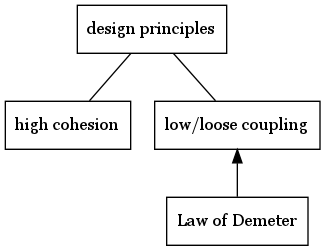
\includegraphics[width=0.5\textwidth]{./graphs/oop_design_principles.png}
  \caption{Znázornění analyzovaných návrhových principů.\label{analyzed_principles}}
\end{figure}

% TODO: v rámci každého návrhového principu uvést příklad porušení
% tohoto principu (případně i příklad, který tento princip dodržuje)

% Příklad pravidla:
% ``Třídy z balíčku A nesmí záviset na jiných konkrétních třídách, ale nejvýše na rozhraních balícků B.''
%  (programování proti rozhraní namísto proti kokrétní implementaci)"

\subsubsection{Low coupling/dependency (nízká závislost/vazba)}
Důležitou návrhovou zásadou je snaha snížit provázanost modulů na minimum. Je možné kategorizovat způsob provázanosti modulů do různých skupin. Následující přehled je převzat z \cite{wiki:coupling} (ještě jemnější dělení je uváděno v \cite{STVR:STVR162}).

\begin{itemize}
\item\emph{Content coupling (nejvyšší forma závislosti)} -- závislost na obsahu modulu -- jeden modul modifikuje nebo se spoléhá na vnitřní fungování jiného modulu (např. přístup k lokálním datům jiného modulu). V důsledku platí, že změní-li se způsob, kterým tento druhý modul produkuje data (umístění, typ, časování), povede to zcela jiste ke změnám v závislém modulu.
\item\emph{Common coupling} -- dva moduly sdílí stejná globální data (např. globální proměnnou), změna sdíleného globálního zdroje implikuje změny všech modulů, které je používají.
\item\emph{External coupling} -- dva moduly sdílí externě definovaný (standardizovaný) datový formát, komunikační protokol nebo rozraní zařízení.
\item\emph{Control coupling} -- jeden modul kontroluje tok druhého tím, že mu posílá informaci o tom, co má konat (např. předání \uv{to-do} příznaku).
  % TODO: CLARIFY
\item\emph{Stamp coupling (Data-structured coupling)} -- mdouly sdílí složenou datovou strukturu a používají pouze její (často odlišnou) část (např. předávání kompletního záznamu funkci, která z něj potřebuje pouze jedno pole). Tato vazba může vést ke změně způsobu, kterým modul čte záznam, protože pole, které tento modul nepotřebuje bylo modifikováno.
  % Stamp coupling is when modules share a composite data structure and use only a part of it, possibly a different part (e.g., passing a whole record to a function that only needs one field of it). This may lead to changing the way a module reads a record because a field that the module doesn't need has been modified.
\item\emph{Data coupling} -- moduly sdílí data pomocí parametrů. Každý parametr je elementární datový typ a jedná se o jediná data, která jsou sdílená (např. předávání celočíselné hodnoty funkci, která spočítá jeho druhou mocninu).
\item\emph{Message coupling (nejnižší forma závislosti)} -- provázanost modulů pouze pomocí zpráv, jedná se o nejnižší úroveň závislosti. Lze jí dosáhnout pomocí decentralizace stavu (u objektů), kde je komunikace dosahováno pomocí parametrů nebo předávání zpráv (\uv{message passing}).
\item\emph{No coupling} -- žádná závislost -- moduly spolu vůbec nekomunikují.
\end{itemize}

%% TODO: sort
%% ## Typy závislostí mezi třídami

%% * třída A dědí ze třídy B
%% * třída A provádí instanciaci třídy B
%% * třída A používá existující intanci třídy B (pracuje s referencí na tuto třídu)

%% Na základě těchto závislostí lze sestavit orientovaný graf. Hrany budeme dále klasifikovat podle toho, o jakou závislost se jedná (dědičnost vs. vyvolání metody).

\subsubsection{High cohesion}
Článek \cite{ISI:000079726000029} uvádí dělení koheze podle tzv SMC\footnote{Podle původních autorů Stevens, Myers a Constantine.} Cohesion:
\begin{enumerate}
\item \emph{Coincidental association} -- there is no relationship between the processing elements.
\item \emph{Logical association} -- both processing elements belong to the same logical class of related functions.
\item \emph{Temporal association} -- each occurrence of both processing elements occurs within the same limited period of time during execution.
\item \emph{Procedural association} -- both processing elements are elements of a common procedural unit which is an iteration or decision process.
\item \emph{Communicational association} -- both processing elements operate upon the same input data set and/or produce the same output data.
\item \emph{Sequential association} -- the output data from one processing element is input to the other processing element.
\item \emph{Functional association} -- both processing elements are essential to the performance of a single function.
\end{enumerate}


\subsubsection{Law of Demeter}

Existuje několik forem Demeterova zákona \cite{35588}, které jsou vhodné pro různé oblasti aplikace. Tyto typy jsou znázorněny na obrázku \ref{demeter_law_types}.

\begin{figure}[h!]
  \centering
  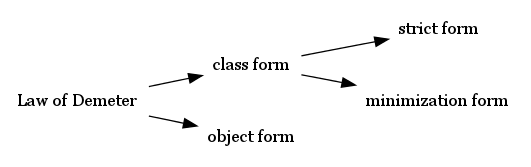
\includegraphics[width=0.7\textwidth]{./graphs/demeter_law_types.png}
  \caption{Formy Demeterova zákona.\label{demeter_law_types}}
\end{figure}

Pro statickou analýzu lze použít \uv{class} formu Demeterova zákona.

\subsection{Ukázky kódu porušujících některá z pravidel}

\subsubsection{Porušení principu law of Demeter}

%% TODO: use some highlighter
%% TODO: add example of demeter law violation from paper notes
\begin{verbatim}
package handlers;

public class ...

\end{verbatim}

\section{Analýza problematiky v jazyce Java}

\subsection{Statický model programu v Javě}
TODO: pojednání o tom, co všechno může být modelem programu (ast, graf, FSM, programovací jazyky, atd)

TODO: možná přidat poznámku o model driven engineering a jak může být aplikováno právě zde

\subsubsection{Struktura softwarového projektu v Javě}

% TODO: sort and rephrase
\begin{itemize}
\item\verb+*.java+ soubory - v gramatice programovacího jazyka Java 1.5 představují top-level element CompilationUnit \emph{\{(TODO: binární součásti projektu? class files?)\}}
\item další soubory - resources, documentation, \ldots
\end{itemize}

Pro naše potřeby jsou důležité v podstatě pouze kompilační jednotky (java soubory) projektu.

Statický pohled na program - neuvažujeme běh programu. Pracujeme nad definicemi tříd, nikoliv nad jejich instancemi v paměti JVM.

% TODO: aktualizovat -> v konecnem dusledku budeme pracovat i nad projekty v jazyku 1.6 (protoze nam to rozhrani umoznuje)
Budeme pracovat nad gramatikou jazyka Java 1.5. Java verze 6 se liší pouze úpravou standardních API poskytovaných platformou Java. Jazyk jako takový zůstává stejný.

\subsubsection{Syntaktické elementy programovacího jazyka Java}
Grafické znázornění základních syntaktických elementů, jejichž struktura a názvy jsou převzaty z \cite{Gosling:2005:JLS:1036643}, je na obrázku \ref{toplevel_elements}.
% TODO: write some better accompanying text
\begin{figure}[h!]
  \centering
  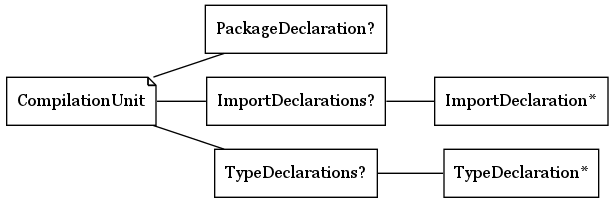
\includegraphics[width=\textwidth]{./graphs/java_top_elements.png}
  \caption{Struktura základních syntaktických elementů programovacího jazyka Java.\label{toplevel_elements}}
\end{figure}

Pro analýzu založenou na vyhledávání závislostí mezi třídami pro nás bude nejdůležitější syntaktický element \emph{TypeDeclaration}. Tento neterminální symbol se dále přepisuje na symboly uvedené na obrázku \ref{type_declaration_options}.

\begin{figure}[h!]
  \centering
  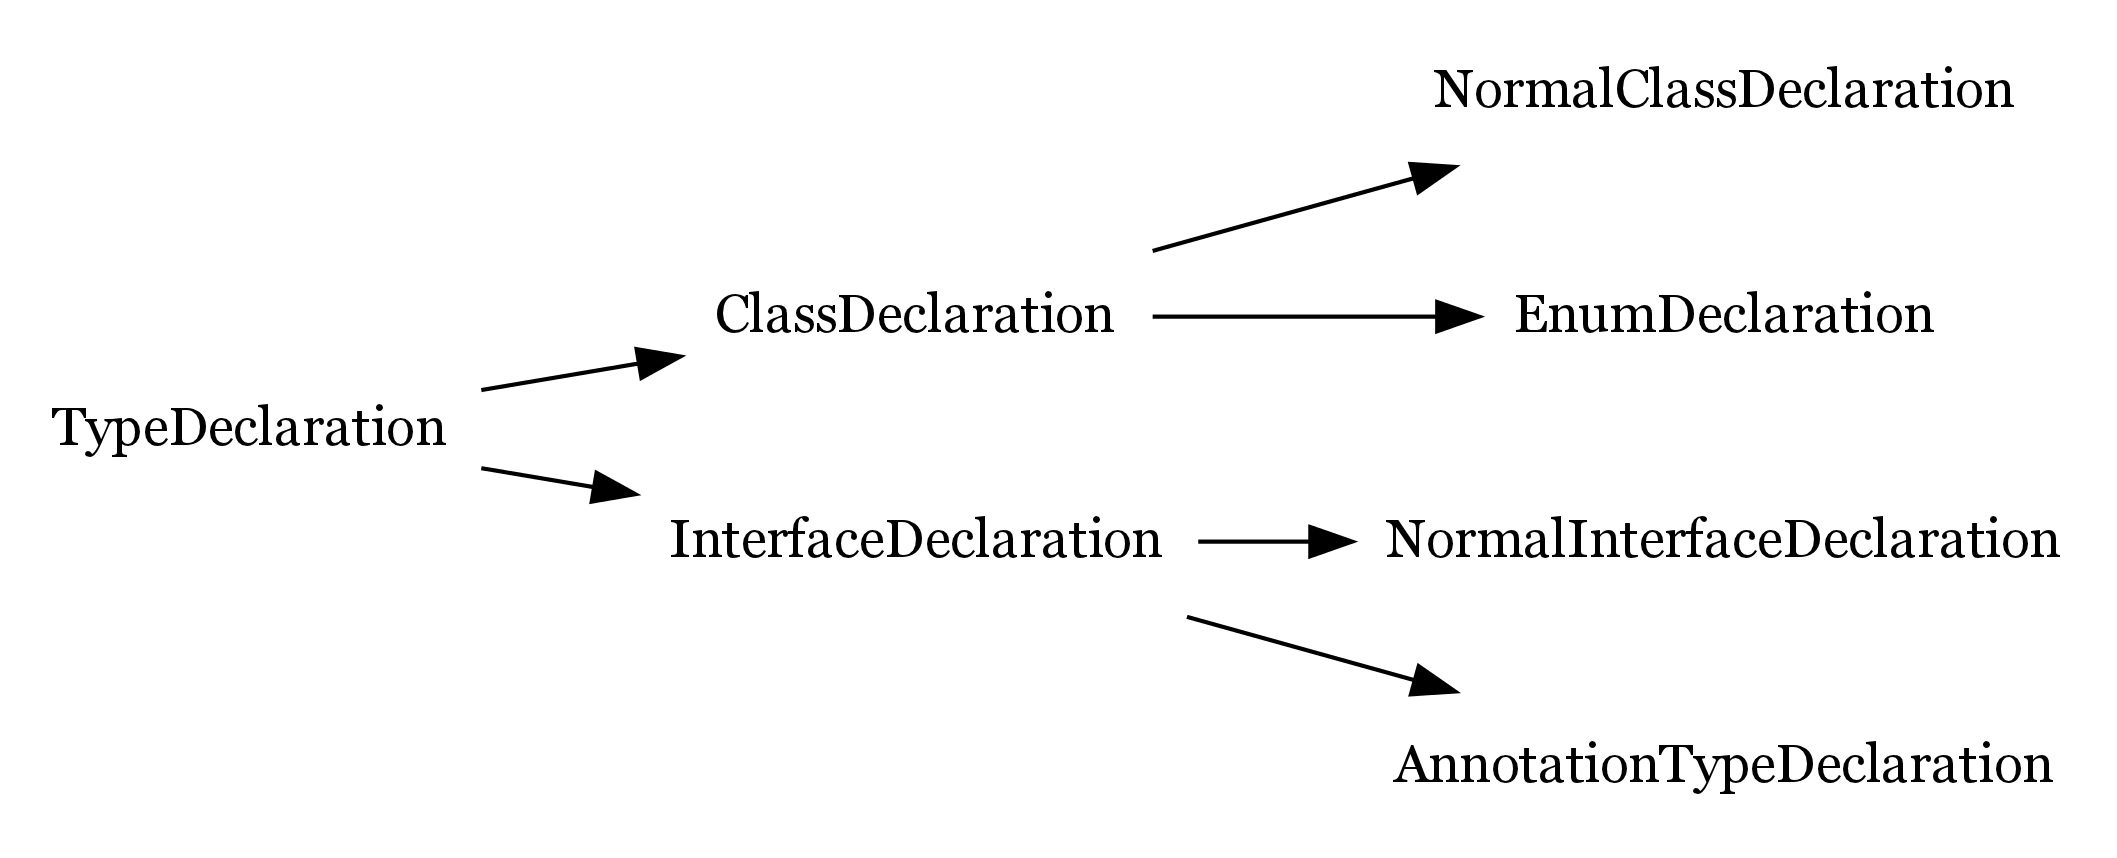
\includegraphics[width=\textwidth]{./graphs/toplevel_types.png}
  \caption{Rozklad elementu TypeDeclaration.\label{type_declaration_options}}
\end{figure}

%% TODO: zatridit tyto syntakticke elementy, ke kazdemu napsat, jak se bude zpracovavat
%% interfaces
%% enums
%% annotations

%% Modifikátory přístupu (private, public, protected, package private) nám umožní "ořezat" graf závislosti tříd. Je ale možné, že pro některé druhy analýzy bude toto nežádoucí.

%% ## Speciální případy:

%% * statické třídy
%% * statické metody
%% * vnitřní třídy

\subsection{Existující nástroje pro zpracování zdrojových kódů v jazyku Java}

TODO: write some leading text

Možnosti zpracovávání kódu:

TODO: roztřídit a vyházet nesmysly (e.g. JABA, apod.)

TODO: použít jinou vhodnější strukturu místo itemize

\begin{itemize}
\item vlastní hand-written lexikální a syntaktický analyzátor (zbytečně náročné)
\item parser vygenerovaný pomocí některého z dostupných compiler-compiler systémů
  \begin{itemize}
  \item tyto systémy na základě vstupní gramatiky vygenerují frontend pro překladač
  \item lze specifikovat různé akce, které jsou navázány na události vyvolané v průběhu syntaktické analýzy
  \item \emph{JavaCC}
    \begin{itemize}
    \item \href{http://www.cs.purdue.edu/homes/hosking/352/javaccdocs/docindex.html}{http://www.cs.purdue.edu/homes/hosking/352/javaccdocs/docindex.html}
    \end{itemize}
  \item \emph{JastAdd}
    \begin{itemize}
    \item \href{http://jastadd.org/}{http://jastadd.org/}
    \end{itemize}
  \item \emph{JLex}
    \begin{itemize}
    \item A Lexical Analyzer Generator for Java(TM)
    \item \href{http://www.cs.princeton.edu/~appel/modern/java/JLex/}{http://www.cs.princeton.edu/~appel/modern/java/JLex/}
    \end{itemize}
  \item JFlex
    \begin{itemize}
    \item The Fast Scanner Generator for Java
    \item \href{http://jflex.de/}{http://jflex.de/}
    \end{itemize}
  \item JABA
    \begin{itemize}
    \item \href{http://pleuma.cc.gatech.edu/aristotle/Tools/jaba.html}{http://pleuma.cc.gatech.edu/aristotle/Tools/jaba.html}
    \item Java Architecture for Bytecode Analysis
    \item nepoužitelné - dostupná pouze binární verze pro Solaris
    \item pravděpodobně se dále nevyvíjí
    \end{itemize}
  \end{itemize}
\item použití vhodné knihovny
  \begin{itemize}
  \item JavaParser
    \begin{itemize}
    \item \href{http://code.google.com/p/javaparser/}{http://code.google.com/p/javaparser/}
    \item projekt na GoogleHosting
    \item v podstatě gramatika pro JJTree vytvářející strom tříd a objektů, který je možné procházet pomocí visitor patternu
    \end{itemize}
  \end{itemize}
\item použití prostředků platformy NetBeans
  \begin{itemize}
  \item Retouche API
  \item \href{http://bits.netbeans.org/6.9.1/javadoc/}{http://bits.netbeans.org/6.9.1/javadoc/}
  \end{itemize}
\item použití prostředků poskytovaných platformou Java 6 (Sun verze) \cite{source_code_analysis_corejavatechtips}
  \begin{itemize}
  \item \emph{JSR 199 -- Java Compiler API}
    \begin{itemize}
    \item volání překladače jazyka Java pomocí API ze zdrojového kódu programu
    \item balíček \verb+javax.tools+
    \end{itemize}
  \item \emph{JSR 269 -- Pluggable Annotation Processing API}
    \begin{itemize}
    \item možnost přidání vlastního kódu pro zpracovávání anotací/kódu do instance překladače
    \item balíček \verb+javax.annotation.processing+ -- zpracovávání anotací
    \item balíček \verb+javax.lang.model+ -- třídy poskytující model pro syntaktické elementy jazyka Java
    \end{itemize}
  \item \emph{Compiler Tree API}
    \begin{itemize}
    \item nestandardní rozšíření Java JDK
    \item \href{http://download.oracle.com/javase/6/docs/jdk/api/javac/tree/index.html}{http://download.oracle.com/javase/6/docs/jdk/api/javac/tree/index.html}
    \item balíček \verb+com.sun.source.tree+ -- poskytuje rozhraní pro reprezentaci zdrojového kódu jako AST
    \item balíček \verb+com.sun.source.util+ -- poskytuje rozhraní pro operace nad AST
    \end{itemize}
  \end{itemize}
\end{itemize}

\chapter{Návrh}

\section{Návrh způsobu specifikace pravidel}

Abychom mohli specifikovat pravidla, musíme nejprve definovat strukturu, nad kterou budou tato pravidla platit. V tomto textu formalizujeme model programu pomocí teorie grafů. Nad grafem je možné dále specifikovat pravidla, která musí vstupní projekt splňovat.

\subsection{Formalizace modelu programu pomocí grafu}
\label{design-graph_formalization}

Analyzovaný softwarový projekt abstrahujeme jako orientovaný multigraf rozšířený o zobrazení množiny uzlů do množiny typů a zobrazení hran do množiny jejich klasifikátorů (označení typu vztahu mezi uzly). Získáme tak následující strukturu:

\begin{displaymath}
G = \langle V, E, \rho, K, C, \mathit{Kind}, \mathit{Class}\rangle
\label{extended_multigraph}
\end{displaymath}
v níž platí:
\begin{itemize}
\item $V$ je množina elementů (v našem případě části kódu)
\item $E$ je množina hran (v našem případě vztahy mezi částmi kódu - např. volání funkce, dědičnost)
\item $V \cap E = \emptyset$
\item $\rho: E \mapsto V \times V$ je zobrazení množiny hran do množiny uspořádaných dvojic vrcholů (incidence)
\item $K$ je libovolná množina označení typů vrcholů\footnote{Pod pojmem typ zde rozumíme jakékoliv označení, které specifikuje o jaký objekt se jedná -- může to být třída, metoda, příkaz, \ldots},
\item $\mathit{Kind}: V \mapsto K$ je zobrazení, které přiřadí každému vrcholu jeho typ,
\item $C$ je množina klasifikátorů hran,
\item $\mathit{Class}: E \mapsto C$ je zobrazení, které přiřadí každé hraně její klasifikátor (zda se jedná o \emph{method call}, \emph{dědičnost}, atd.)
\end{itemize}

Ukázka formalizace zdrojového kódu pomocí grafu je na obrázku \ref{design-graph_example}. V uvedeném příkladě můžeme strukturu $G$ namapovat následujícím způsobem:
\begin{figure}[h!]
  \centering
  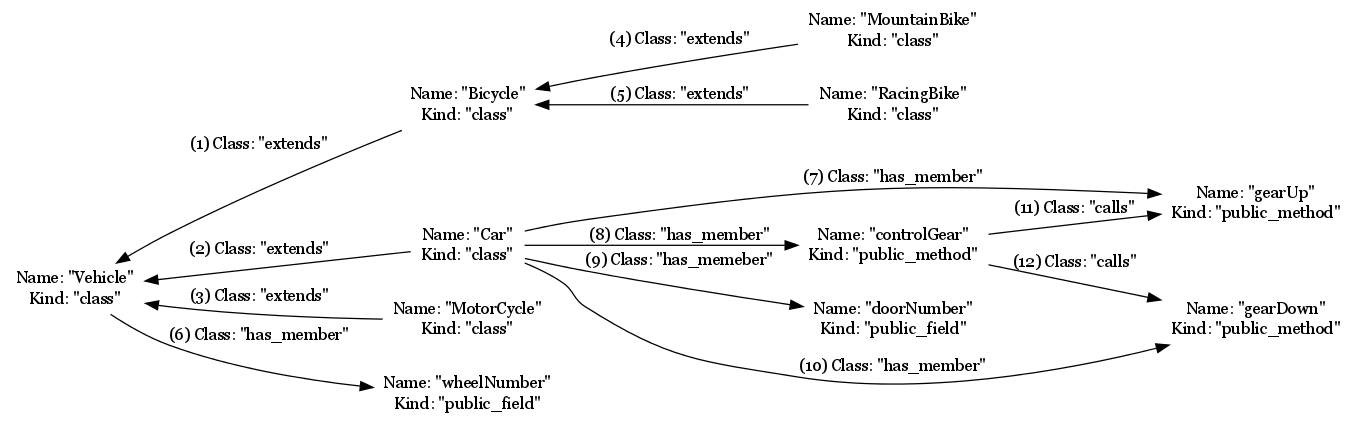
\includegraphics[width=1.0\textwidth]{./graphs/graph_example.png}
  \caption{Příklad formalizace hierarchie tříd jako grafu.\label{design-graph_example}}
\end{figure}
Množinu vrcholů můžeme ztotožnit s množinou názvů elementů (v našem případě třídy, pole, metody).
\begin{align*}
V = &\{ \\
&Vehicle, Car, MotorCycle, Bicycle, MountainBike, RacingBike, \\
&wheelNumber, doorNumber, \\
&controlGear, gearUp, gearDown \\
&\}
\end{align*}
Abychom mohli demonstrovat množinu hran, bylo provedeno očíslování. Hranu zde identifikujeme číslem. V počítačové reprezentaci se může jednat o konkrétní objekt uložený v poli. Množinu hran potom můžeme reprezentovat prostým výčtem čísel:
\begin{displaymath}
E = \{1, 2, 3, 4, 5, 6, 7, 8, 9, 10, 11, 12\}
\end{displaymath}
Zobrazení $\rho$ můžeme formálně zapsat jako následující množinu\footnote{Zobrazení je binární relace. Proto jej můžeme reprezentovat jako množinu uspořádaných dvojic.}:
\begin{align*}
\rho = &\{ \\
&(1, (Bicycle, Vehicle)), \\
&(2, (Car, Vehicle)), \\
&(3, (MotorCycle, Vehicle)), \\
&(4, (MountainBike, Bicycle)), \\
&(5, (RacingBike, Bicycle)), \\
&(6, (Vehicle, wheelNumber)), \\
&(7, (Car, gearUp)), \\
&(8, Car, controlGear)), \\
&(9, (Car, doorNumber)), \\
&(10, (Car, gearDown)), \\
&(11, (controlGear, gearUp)), \\
&(12, (controlGear, gearDown)) \\
&\}
\end{align*}
Zbývají nám množina typů $K$,
\begin{align*}
K = \{ class, public\_field, public\_method \}
\end{align*}
množina klasifikátorů hran $C$,
\begin{align*}
C = \{ \langle\langle{}extends\rangle\rangle, \langle\langle{}has\_member\rangle\rangle, \langle\langle{}calls\rangle\rangle \}
\end{align*}
přiřazení typů uzlům $Kind$,
\begin{align*}
Kind = &\{ \\
&(Bicycle, class), \\
&(Car, class), \\
&(MotorCycle, class), \\
&(MountainBike, class), \\
&(RacingBike, class), \\
&(Vehicle, class), \\
&(wheelNumber, public\_field), \\
&(doorNumber, public\_field), \\
&(controlGear, public\_method), \\
&(gearUp, public\_method), \\
&(gearDown, public\_method) \\
&\}
\end{align*}
a přiřazení klasifikátorů hranám:
\begin{align*}
Class = &\{ \\
&(1, \langle\langle{}extends\rangle\rangle), \\
&(2, \langle\langle{}extends\rangle\rangle), \\
&(3, \langle\langle{}extends\rangle\rangle), \\
&(4, \langle\langle{}extends\rangle\rangle), \\
&(5, \langle\langle{}extends\rangle\rangle), \\
&(6, \langle\langle{}has\_member\rangle\rangle), \\
&(7, \langle\langle{}has\_member\rangle\rangle), \\
&(8, \langle\langle{}has\_member\rangle\rangle), \\
&(9, \langle\langle{}has\_memeber\rangle\rangle), \\
&(10, \langle\langle{}has\_member\rangle\rangle), \\
&(11, \langle\langle{}calls\rangle\rangle), \\
&(12, \langle\langle{}calls\rangle\rangle), \\
\}
\end{align*}

%% Graf elementů použitých v kódu. Vrcholy $v \in V$ představují různé syntaktické elementy v analyzovaném kódu. Záleží na úrovni prováděné analýzy, jaké zvolíme vrcholy. V případě, že budeme analyzovat \uv{nízkoúrovňové} chování funkce, mohou být vrcholy jednotlivé příkazy a jejich části. Pokud budeme analyzovat míru provázanosti tříd nebo metod, stačí když použijeme jako vrcholy třídy a metody (případně parametry metod.)
%% $G = (V, E)$

\subsection{Formalizace pravidel}

\begin{itemize}
\item definice jazyka pro specifikaci pravidel
\item specifikovat množinu objektů, nad nimiž budou pravidla stavěna -- nad čím budeme operovat (možnosti: gramatika, třídy, FJ, graf, \ldots)
\item lze vyjít z Java Language Specification (množina neterminálních a terminálních symbolů)
\item může být nějaký DSL
\end{itemize}

\subsection{Typy pravidel}
\begin{itemize}
\item pravidla definovaná ve vytvořeném formalismu (DSL rules)
\item uživatelsky programovaná pravidla (custom code java code, asserts)
\end{itemize}

TODO: zapracovat:

Ne všechna pravidla lze popsat exaktně ve smyslu splněno/nesplněno. Mnohdy můžeme kvalitu návrhu posuzovat pouze kvantitativně (dobrý návrh, lepší, moc vazeb, málo vazeb, atd.). Pro některé vlastnosti návrhu (např. low coupling, high cohesion) může být vhodnější poskytnou statistický přístup pro vyhodnocování (např. použití vhodného klasifikátoru).

\section{Návrh architektury systému}
TODO: highlevel design $\rightarrow$ jaké budou moduly a co budou dělat (zatím bez konkrétní použité technologie)

% NOTE: při zpracování většího projektu bude nejspíš nutné zavést nad jmény objektů vhodnou formu indexace pro zrychlení algoritmů (kanonická jména tříd jsou v javě poměrně dost dlouhá)

\begin{itemize}
\item compiler
\item generátor vnitřní struktury (modelu) -- modelem je v našem případě graf
\begin{itemize}
\item \emph{vstup:} množina cest k \verb+*.java+ souborům (kompilačním jednotkám), z nichž se skládá softwarový projekt
\item \emph{výstup:} graf, reprezentující konkrétní analyzovanou doménu vhodný pro další zpracování (graf podle \ref{design-graph_formalization} \nameref{design-graph_formalization})
\end{itemize}
\item možnosti generování grafu závislostí mezi třídami (vnitřní reprezentace):
  \begin{itemize}
  \item on demand -- když bude potřeba, vybuduje se kompletně celý graf a poté se zahodí
  \item on the fly -- při práci uživatele na kódu se bude vždy generovat znovu celý graf
  \item kombinovaný přístup -- graf se ve vhodných okamžicích celý vybuduje a poté budou probíhat jeho následné aktualizace na základě uživatelovy práce nad kódem
  \end{itemize}
\item analyzátor
\item rozhraní - integrace do platformy NetBeans
  \begin{itemize}
  \item rozhraní pro zadávání pravidel
  \item rozhraní pro ověřování platnosti pravidel (validaci)
  \end{itemize}
\end{itemize}

% TODO: navrhnout aplikaci tak, aby mela vice rozhrani (nejen GUI, ale i moznost integrace, moznost textoveho vstupu pravidel)

\section{Návrh rozhraní pro zadávání pravidel}
%% rozhraní pro zadávání pravidel bude dáno jazykem, který se pro definici pravidel bude používat - možná kompilátor DSL jazyka, výrazy, atd.
\begin{itemize}
\item rozhraní pro zadávání pravidel
\item formát zadávání pravidel (serializace formalismu tak, aby jej bylo možné textově nebo jinak zadávat)
\end{itemize}

\section{Návrh rozhraní pro ověřování platnosti pravidel (validaci)}
\begin{itemize}
\item výstupní rozhraní
\item validační události
\end{itemize}

%% TODO:
% typy grafů: class hierarchy graph, call graph
% call graph: wikipedia (<<invokes>> vazby)
%
% http://en.wikipedia.org/wiki/Call_graph
%

\chapter{Implementace}
\label{implementation}
\emph{Implementační} část práce se skládala z~několika součástí. Za nejvýznamnější součást lze považovat formální specifikaci pravidla \emph{Law of Demeter}, která je uváděna jako první v~rámci této sekce. V~dalších částech kapitoly se potom zabýváme vybranými poznámkami z~implementace jádra systému \emph{ArchVal}, který má sloužit jako platforma pro provádění matematických formulací návrhových pravidel a implementací rozšíření tohoto systému. V~poslední části je rozebírán způsob integrace systému do platformy NetBeans.

\section{Specifikace pravidel požadovaných zadáním práce}
Nejprve definujeme vhodné operátory, které nám umožní vybrat množiny vrcholů tak, abychom mohli specifikovat \emph{LoD}. Vybrané množiny potom ověříme pomocí predikátu, který určí, zda jsou tyto množiny v~pořádku, či zda porušují \emph{LoD} princip.

\begin{definition}
Mějme grafový model projektu $G = \langle V, E, \rho, K, C, N, \mathit{Kind}, \mathit{Classifier}, \mathit{Name}\rangle$. Definujme selektor vrcholů $L_0(G, v', c')$, $v' \in V$, $c' \in C$ jako množinu vrcholů $v \in V$, které jsou přímými následníky vrcholu $v'$, do kterých se dostaneme po hraně $e \in E$, pro kterou platí $Classifier(e) = c' $.
\end{definition}

\begin{definition}
Mějme grafový model projektu $G = \langle V, E, \rho, K, C, N, \mathit{Kind}, \mathit{Classifier}, \mathit{Name}\rangle$. Definujme selektor vrcholů $L_1(G, v', c_1, c_2)$, $v' \in V$, $c_1 \in C$, $c_2 \in C$ jako množinu vrcholů $v \in V$, do nichž se dostaneme z~vrcholu $v'$ po orientované cestě délky 2, pro jejíž první hranu $e_1$ platí $Classifier(e_1) = c_1$ a pro druhou hranu $e_2$ platí $Classifier(e_2) = c_2$.
\end{definition}

\subsection{Law of Demeter}
\label{implementation-lod_specification}
Pro definici princip \emph{LoD} si zavedeme speciální typ grafového modelu. Ačkoliv jsme pojem \emph{typ grafového modelu}  přesně nedefinovali a zavedli jej pouze intuitivně, pokusíme se nyní vymezit pojem \emph{demeter graph model}, který zde budeme dále používat, přesněji.

U~grafového modelu typu \emph{Demeter graph type} povolíme libovolná označení vrcholů (konkrétně pro potřeby \emph{LoD} se bude jednat o~plně kvalifikované názvy tříd a metod). Množinu typů vrcholů omezíme na následující množinu:
\begin{align*}
K = \{ ``class", ``method" \}
\end{align*}
Význam těchto typů je zřejmý. Typ \emph{class} použijeme pro vrcholy, které budou odpovídat deklarovaným třídám v~existujícím projektu a typ \emph{method} bude označovat jejich metody.

Taktéž množina klasifikátorů hran nebude libovolná, ale bude přesně daná:
\begin{align*}
C = \{ ``field", ``self", ``arg", ``constr", ``use" \}
\end{align*}
Podívejme se na význam těchto označení:
\begin{itemize}
\item $``field"$ -- hrana vede do třídy, které reprezentuje třídní proměnnou nebo do její nadtřídy,
\item $``self"$ -- hrana vede do třídy, která je vlastníkem této metody nebo do její nadtřídy,
\item $``arg"$ -- hrana vede do třídy argumentu metody nebo do její nadtřídy,
\item $``constr"$ -- hrana vede do třídy použité pro konstrukci nového objektu v~těle metody nebo do její nadtřídy,
\item $``use"$ -- hrana vede do třídy, jejíž použití (vyvolání metody nebo přístup k~poli) se vyskytuje v~těle metody.
\end{itemize}
Je patrné, že tyto hrany zčásti odpovídají požadavkům \emph{LoD}. Prozatím jsme uvedli množiny klasifikátorů bez vymezení, kde lze přesně tyto klasifikátory použít. Uvažujme následující množinu, která reprezentuje zobrazení množiny klasifikátorů do množiny dvojic typů vrcholů:
\begin{align*}
GT = &\{ \\
&(``field" (``class", ``class")), \\
&(``self" (``method", ``class")), \\
&(``arg" (``method", ``class")), \\
&(``constr" (``method", ``class")), \\
&(``use" (``method", ``class")) \\
&\}
\end{align*}
Pokud budeme uvažovat koncové vrcholy jednotlivých hran a jejich zobrazení do množiny typů, potom musí platit, že obraz jednotlivých komponent hrany (vrcholů) bude shodný s~obrazem hrany provedeného pomocí zobrazení GT.

Pokud \emph{grafový model projektu} splní všechny tyto podmínky, řekneme o~něm, že je typu \emph{demeter}.

Příklad takového grafu je na obrázku \ref{implementation-lod_graph}. V~uvedeném obrázku princip \emph{LoD} porušuje metoda \verb-method1_2-, která používá třídu \verb-Class2-, ačkoliv není ani jednou z~dovolených tříd principu \emph{LoD} (třída pole vlastnické třídy metody, argument metody, atd.).

\begin{figure}[h!]
  \centering
  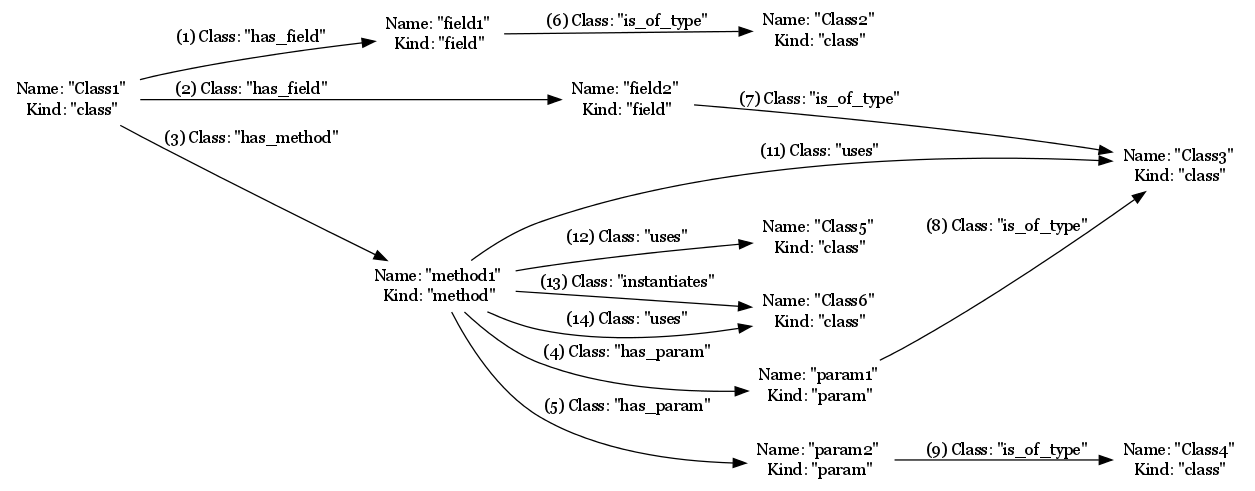
\includegraphics[width=1.0\textwidth]{./graphs/demeter_graph.png}
  \caption{Graf \uv{typu demeter} použitý pro validaci principu \emph{LoD}.\label{implementation-lod_graph}}
\end{figure}

\begin{designprinciple}
Mějme grafový model projektu $G = \langle V, E, \rho, K, C, \mathit{Kind}, \mathit{Classifier}\rangle$ typu demeter. Model $G$ splňuje návrhový princip \emph{LoD}, pokud pro něj platí:

\begin{align*}
\forall v \in V: Kind(v) = ``method"\\
\end{align*}
\begin{align*}
&L_0(G, v, ``use") \setminus (G, L_0(v, ``self") \cup L_1(G, v, ``self", ``field") \cup \\
&L_0(G, v, ``arg") \cup L_0(G, v, ``constr")) = \emptyset
\end{align*}

\end{designprinciple}

Specifikované pravidlo vyjadřuje požadavek, aby množina vrcholů (představujících třídy) do níž se dostaneme pomocí hran s~klasifikátorem $``use"$ (všechna použití tříd uvnitř metody) byla podmnožinou sjednocení vrcholů, které pro danou metodu představují povolená použití tříd (vlastní třída metody, třída třídní proměnné, argument metody nebo konstruovaná třída). Je-li totiž množina $``use"$ vrcholů podmnožinou sjednocení ostatních množin, množinový rozdíl bude roven prázdné množině. V~opačném případě bude množinový rozdíl nenulový, což bude znamenat porušení principu \emph{LoD}.

\subsection{Low coupling, high cohesion}
Zatímco princip \emph{LoD} se nám podařilo přesně specifikovat pomocí množin. U~principů \emph{low coupling} a \emph{high cohesion} bychom spíše uvažovali o~realizaci vhodné analýzy. Tyto analýzy však nebyly cílem této práce.

Přesto byla realizována programová podpora, která umožní snadné přidání modulu, který může pracovat nad libovolným grafem poskytovaným některým z~existujících poskytovatelů generátorů grafů a tyto nebo jiné podobné vlastnosti analyzovat. Většinou by se jednalo o~nejrůznější statistické analýzy založené na počtech hran, seskupování nebo generování histogramů.

Konkrétní informace a rešerše týkající se těchto principů byly rozebrány v~kapitole \ref{analysis}.

\section{Implementace jádra systému}
Jádro systému bylo implementováno v~rámci samostatného modulu platformy NetBeans. Ačkoliv je takto svázáno s~konkrétní platformou, zdrojové kódy neobsahují žádné závislosti na prvky této platformy a je tedy možné je znovupoužít v~jiných projektech.

V~této sekci nebudeme procházet úplně všechny implementované komponenty systému. Jednak byly popsány již v~části návrhu a kromě toho jsou jejich implementace k~dispozici v~rámci zdrojových kódů. Při implementaci byla snaha o~maximální zdokumentovanost -- většina klíčových tříd je řádně opatřena dokumentací \verb-javadoc-.

Zde se podíváme na implementaci formátu pro zadávání pravidel (AVD specifikace). Dále na způsob sestavování vyhodnocovacího stromu a nakonec ukážeme implementaci zajímavých operátorů, které jsou základem systému pro vyhodnocování pravidel.

\subsection{Implementace formátu AVD}
Formát AVD byl vytvořen snahou o~namapování dříve definovaných matematických výrazů do vhodné serializace. Pro zpracování existujícího souboru byl použit lexikální a syntaktický analyzátor vygenerovaný pomocí nástroje ANTLR. Tento nástroj umí kromě vytvoření čistého \emph{parse tree} vytvořit i vhodný AST pomocí jednoduchých přepisovacích pravidel (konkrétní příklady pravidel si můžete prohlédnout v~příloze \ref{avd_grammar}, kde je pro refrenci uvedena celá vstupní gramatika pro nástroj ANTLR).

V~rámci AVD specifikace bylo nutné definovat několik nezávislých jmenných prostorů:

\begin{itemize}
\item názvy analýz,
\item jména typů grafů,
\item jména atomických a složených pravidel (jmenný prostor pro atomická i složená pravidla je sdílený),
\item jména operátorů.
\end{itemize}

Proto je například možné použít stejný název pro typ grafu a pro atomické pravidlo, ale není možné použít shodný název pro dvě pravidla (ať už atomická nebo složená).

\subsection{Implementace sestavování validačního modelu}
Na základě AST, který byl získán pomocí syntaktického parseru vygenerovaného pomocí nástroje ANTLR byl postupně budován vyhodnocovací strom odpovídající zpracovávanému AVD souboru.

Zpracování AST probíhá tím způsobem, že je nejprve zkontrolována bezkoliznost použitých jmen (viz výše zmíněné jmenné prostory). Následně jsou procházeny jednotlivé listy představující pravidla a jsou postupně doplňovány názvy nalezených pravidel do tabulky symbolů. Pro každé pravidlo je nutné sestoupit do syntaktických stromů představujících např. logické výrazy a pro každý takto nalezených vrchol (např. operátor \verb+OR+) je nutné vytvořit nový vrchol vyhodnocovacího stromu.

Tyto nově vytvářené vrcholy jsou realizované pro základní operátory jako samostatné třídy. Pro uživatelské operátory potom existují vrcholy, kterým je při konstrukci možné nastavit operátor, který mají provádět. Předtím, než jsou ale tyto vrcholy vytvořeny, je provedena kontrola, zda počty argumentů a návratová hodnota odpovídá očekávaným hodnotám (např. při zpracování predikátu kontrolujeme, zda množina operandů odpovídá množině deklarované operátorem nalezeným v~registru operátorů.).

Při budování stromu je současně budována infrastruktura pro generování stromu výsledků. V~každém přidávaném vrcholu (představován třídou) je tedy již přítomen kód, který při vyhodnocení uzlu (metoda \verb-evaluate()-) naplní datovou strukturu předanou jako parametr.

\subsection{Implementace základních operátorů}
V~této podsekci se podíváme na některé zajímavé operátory a jejich implementaci. Konkrétně na existenční $\exists$ a univerzální $\forall$ kvantifikátor.

Vyhodnocení univerzálního kvantifikátoru $\forall v \in V$ lze přepsat jako jednoduchý cyklus přes vrcholy vrácené zpřesňující operátorem, která vybírá nějakou podmnožinu z~množiny vrcholů analyzovaného grafu. Získáme tak kód podobný výpisu \ref{listing-forall}. V~tomto kódu, který je fragmentem metody, používáme symbolický název \verb+condition+ pro podmínku, kterou musí splňovat každý prvek \emph{v} iterované kolekce vrcholů \emph{vertices}.
\vspace{0.5cm}
\begin{lstlisting}[
    language=java,
    caption={Implementace univerzálního kvantifikátoru $\forall$.},
    label=listing-forall
  ]
for (Vertex v : vertices) {
    if (!condition(v, ...)) {
        return false;
    }
}
return true;
\end{lstlisting}

Analogicky budeme postupovat u~existenčního kvantifikátoru $\exists$. Zde nám stačí nalézt alespoň jeden element, pro který vyhodnocovaná vlastnost platí. Výpis \ref{listing-exists} představuje fragment metody. Pokud se podaří nalézt alespoň jeden prvek, který splňuje požadovanou podmínku, metoda vrátí hodnotu \emph{true}. Vzhledem k~použití příkazu \emph{return} je zřejmé, že dochází k~\uv{línému} vyhodnocování -- vyhodnocení je ukončeno nalezením prvního vyhovujícího elementu (další se neprohledávají). Stejně jako u~operátoru $\forall$ i zde název \verb+condition+ symbolizuje konkrétní podmínku, která má platit nad alespoň jedním prvkem množiny uzlů.

\vspace{0.5cm}
\begin{lstlisting}[
    language=java,
    caption={Implementace existenčního kvantifikátoru $\exists$.},
    label=listing-exists
  ]
for (Vertex v : vertices) {
    if (condition(v, ...)) {
        return true;
    }
}
return false;
\end{lstlisting}

Můžeme si všimnout, že se obě implementace liší pouze přehozením podmínek -- zatímco v~prvním případě ($\forall$) musíme projít všechny prvky, abychom zjistili, zda všechny prvky splňují požadovanou vlastnost, ve druhém případě ($\exists$) budeme všechny prvky procházet pouze v~krajním případě, kdy vlastnost neplatí pro žádný z~prvků.

Podobným způsobem jsou realizovány i další operátory. Například sjednocení množin využívá operací poskytovaných třídou \verb-HashSet- programovacího jazyka Java.

\section{Implementace modulů rozšíření}
V~rámci této práce byly realizovány celkem dva NetBeans moduly realizující rozšíření. Tyto moduly mohou současně sloužit jako návod k~implementaci dalších rozšíření. Jedná se o~poskytovatele generátoru grafu typu \emph{demeter} a balíček operátorů, které jsou nezbytné k~provedení pravidla \emph{LoD}. Tyto operátory nicméně nejsou vázány pouze na princip \emph{Law of Demeter}. Například operátor, který testuje, zda je množina vrcholů prázdná má zcela jistě obecné použití.

\subsection{Modul av-graphgen-demeter (generátor grafu)}
Modul pro generování grafu nad nímž je možné provést kontrolu principu \emph{LoD}, je realizován díky možnosti využít existující infrastrukturu platformy NetBeans pro práci se zdrojovými kódy v~jazyce Java a jejich syntaktickými stromy. Jak již bylo zmíněno dříve v~rámci analýzy, platforma NetBeans poskytuje AST stromy, které mají již rozlišené symboly. Díky tomu můžeme stromy postupně procházet a dotazovat se na plně kvalifikovaná jména elementů představujících třídy, rozhraní atd.

Generátor grafu je realizován v~rámci třídy \emph{DemeterGraphGenerator} (implementuje rozhraní \emph{GraphGeneratorIface}). Protože vstupním parametrem pro generátor grafu je \uv{pouze} adresář projektu. Je nutné vylistovat všechny soubory, které mohou obsahovat zdrojový kód v~jazyce Java (\verb+*.java+ soubory). Následně je pro každý takový soubor získána instance třídy \emph{JavaSource} poskytované platformou NetBeans. Tato třída je vstupním bodem k~funkcionalitám poskytovaným kompilátorem jazyka Java (třída JavaSource tato rozhraní zabaluje). Díky tomu je možné využít \emph{Java Tree API} pro iteraci všech syntaktických elementů v~rámci kompilační jednotky.

To je provedeno formou návrhového vzoru \emph{Visitor}. Při generování demeter grafu nemusíme naštěstí přepisovat všechny metody třídy \emph{TreePathVisitor}, ale zaměřujeme se pouze na elementy, které potřebujeme pro vygenerování grafu. Pro vygenerování potřebného grafu nám stačí získat následující informace: které třídy je metoda členem, zjištění všech nadtříd třídy, konstrukce nové proměnné (nebo pole proměnných), deklarace polí třídy, vyvolání metody a přístup k~poli třídy. Ostatní syntaktické konstrukce nejsou pro tento druh generování grafu podstatné.

\subsection{Modul av-operators-demeter (operátory pro LoD)}
Balík operátorů poskytovaný modulem \verb+av-operators-demeter+ obsahuje následující operátory:

\begin{itemize}
\item \verb+vertex_set_is_empty+ -- třída \emph{EmptyVertexSetPredicate} -- operátor, který vrátí \verb+true+ v~případě, že je množina vrcholů předaná jako parametr prázdná,
\item \verb+level_zero_vertex_selector+ -- třída \emph{LevelZerorVertexSelector} -- implementace operátoru $L_0$ tak jak byl definován dříve,
\item \verb+level_one_vertex_selector+ -- třída \emph{LevelOneVertexSelector} -- implementace operátoru $L_1$ tak jak byl definován dříve,
\item \verb+kind+ -- třída \emph{VertexKindPredicate} -- predikát, který vrátí \verb+true+, pokud má vrchol předaný jako první parametr typ shodný s~řetězcem předaným jako druhý parametr.
\end{itemize}

Implementace operátorů je poměrně přímočará. Zajímavý je snad jen operátor \emph{F}, který pomocí jednoduché rekurze implementuje modifikované prohledávání do hloubky, aby získal množinu potřebných vrcholů.

\section{Integrace do NetBeans IDE}

Pro demonstraci jádra systému bylo nutné jej zaintegrovat do vhodného běhového prostředí. K~tomu dobře posloužila platforma NetBeans. Při implementaci bylo hojně využíváno informací z~\cite{netbeans_platform}. Integrace byla provedena realizací vhodných integračních komponent v~rámci modulu \verb+av-platform-integration+. Jejich seznam je k~dispozici v~tabulce \ref{implementation-integration_components}.

\begin{table}
  \caption{Tabulka integračních komponent systému. \label{implementation-integration_components}}
  \begin{center}
    \begin{tabular}{ | l | l | p{8cm} | }
      \hline
      \textbf{Název} & \textbf{Typ} & \textbf{Zodpovědnost} \\
      \hline
      \hline
      ArchvalInstance & class (singleton) & zabaluje jednotnou instanci jádra \emph{ArchVal} \\ \hline
      ValidateMainProject & class & integrace s~běhovou platformou, vstupní/aktivační bod \\ \hline
      GraphGeneratorRegister & class & třída poskytující přístup k~informacím o~existujících poskytovatelích generátorů grafu \\ \hline
      OperatorRegister & class & třída poskytující přístup k~informacím o~existujících poskytovatelích operátorů \\ \hline
      AnalysesRegister & class & třída poskytující přístup k~informacím o~existujících poskytovatelích komponent analýzy \\ \hline
    \end{tabular}
  \end{center}
\end{table}

\subsection{Použití jádra systému ArchVal}
Vstupním bodem pro použití rozhraní jádra systému \emph{ArchVal} v~rámci integračního modulu je třída \emph{ArchvalInstance}. Tato třída je implementována jako návrhový vzor \emph{singleton} a poskytuje jedinou instanci třídy \emph{ArchVal} pro celý systém. Díky tomu je možné se dále dostat k~důležitým komponentám jako \emph{ValidationModelGenerator}, \emph{GraphModelGenerator} a vygenerovat instanci \emph{ValidationTask}, která umí provést výslednou validaci.

\subsection{Přidání uživatelské akce do nabídky prostředí}
Aby bylo možné vyvolat validaci, bylo nutné provést integraci akce do nabídky NetBeans IDE. Akce představovaná třídou \emph{ValidateMainProject} byla realizována jako podmíněně povolená akce, která je k~dispozici pouze pokud je vybrán soubor konkrétního typu. V~tomto případě se jedná o~soubor typu AVD. Celý případ užití funguje potom tím způsobem, že uživatel klepne pravým tlačítkem na AVD soubor a vybere položku \emph{Validate main project}. Pokud není žádný projekt vybrán jako hlavní, v~oznamovací oblasti se pouze objeví upozornění a není provedena žádná akce. V~opačném případě máme k~dispozici oba vstupy potřebné k~provedení validace (pomocí \emph{Project API} získáme informace o~hlavním projektu a tedy i vstupním adresáři a cesta k~AVD souboru je poskytována v~rámci handleru kontextové akce AVD souboru).

\subsection{Výstupní rozhraní}
Pro zobrazení výstupu použijeme NetBeans \emph{I/O API}, které nám umožňuje využít jednoduché textové okno, které se používá v~NetBeans IDE například pro zobrazení výstupů z~logu nebo informace o~průběhu kompilace. Poskytované aplikační rozhraní nám umožňuje otevřít novou záložku, kde můžeme samostatně logovat výsledky validační akce. V~základní verzi nástroj implementuje pouze výstup ve tvaru \emph{[název pravidla] OK} nebo \emph{[název pravidla] Violation found.}

\subsection{Implementace registrů poskytovatelů služeb}
Díky systému \emph{Lookup} poskytovanému platformou NetBeans je implementace registrů poskytovatelů služeb velmi pohodlná. Pro každé rozhraní, pro něž chceme využívat \emph{lookup} stačí přidat seznam implementujících tříd do konkrétního souboru v~adresáři \emph{META-INF/services}. Následně pak můžeme využít jednoduché volání pro zisk všech instancí implementujících dané rozhraní v~celém systému:

\begin{verbatim}
Lookup.getDefault().lookupAll(OperatorIface.class)
\end{verbatim}

Zmíněný příklad slouží k~získání všech existujících tříd poskytujících rozhraní operátorů. Získané reference si v~implementovaných registračních třídách ponecháváme uložené v~kolekcích, abychom nemuseli opakovaně vyhledávat instance v~lookupu, zvláště když víme, že tam vzhledem k~jejich povaze žádné nemohou přibýt.

\subsection{Podpora editace AVD souborů}
Pro zjednodušení zadávání AVD souboru byla realizována podpora zvýrazňování syntaxe. Ta je realizována v~rámci samostatného modulu \verb-av-avd-highlighter-, který využívá služeb jádra (ANTLR lexer pro tokenizing AVD souborů). Zvýrazňování syntaxe bylo integrováno do platformy NetBeans pomocí několika jednoduchých adaptérů, které zapouzdřují lexer vygenerovaný pomocí nástroje ANTLR (který se používá již v~modulu \verb+av-core+).

Aby platforma NetBeans mohla soubory rozpoznat a pracovat s~nimi stejně jako s~ostatními datovými uzly, je nutné zaregistrovat do platformy nový typ souboru. Pro potřeby této práce byl použit experimentální MIME typ \verb+text/x-avd+.

\chapter{Testování}

% TODO: na úvod této sekce popsat všechny prováděné testy
% TODO: popsat průběh a výsledky všech typů testování

\begin{itemize}
\item jednotkové testování (unit testing)
\item validace výsledné práce - splňuje práce očekávaný výsledek?
\item testování práce na vstupech různých typů
\item srovnání práce s~existujícími řešeními (\ref{requirements-existing_tools} -- \nameref{requirements-existing_tools})
\end{itemize}

%% \section{Jednotkové testování (unit testing)}

\chapter{Závěr}

\begin{itemize}
\item Zhodnocení splnění cílů DP/BP a  vlastního přínosu práce (při formulaci je třeba vzít v potaz zadání práce).
\item Diskuse dalšího možného pokračování práce.
\end{itemize}


% TODO: complete references
%\bibliographystyle{abbrv}

\bibliographystyle{csplainnat}

%bibliographystyle{plain}
%\bibliographystyle{psc}
{
  %JZ: 11.12.2008 Kdo chce mit v techto ukazkovych odkazech take odkaz na CSTeX:
  \def\CS{$\cal C\kern-0.1667em\lower.5ex\hbox{$\cal S$}\kern-0.075em $}
  \bibliography{reference}
}

% M. Dušek radi:
%\bibliographystyle{alpha}
% kdy citace ma tvar [AutorRok] (napriklad [Cook97]). Sice to asi neni  podle ceske normy (BTW BibTeX stejne neodpovida ceske norme), ale je to nejprehlednejsi.
% 3.5.2009 JZ polemizuje: BibTeX neobvinujte, napiste a poskytnete nam styl (.bst) splnujici citacni normu CSN/ISO.

\appendix

\chapter{Seznam použitých zkratek}

\begin{description}
\item[AST] Abstract Syntax Tree
\end{description}
\vdots

\chapter{UML diagramy}
\textbf{\large Tato příloha není povinná a zřejmě se neobjeví v každé práci. Máte-li ale větší množství podobných diagramů popisujících systém, není nutné všechny umísťovat do hlavního textu, zvláště pokud by to snižovalo jeho čitelnost.}

\chapter{Instalační a uživatelská příručka}

\section{Instalace programu}

K dispozici jsou dvě varianty programu (adresář \verb+dist+ na přiloženém cd). Soubor \verb+archval.zip+ obsahuje spustitelnou variantu projektu. Pro platformu Linux je možné využít instalátor (soubor \verb+achval-linux.sh+).

V případě instalace ze zip soubor stačí tento soubor rozbalit do vhodného umístění. Pro spuštění instalátoru může být nutná nastavit executable bit pomocí příkazu:

\begin{verbatim}
chmod u+x archval-linux.sh
\end{verbatim}

U obou typů instalací je však nutné provést konfiguraci systému v souboru \verb+etc/archval.conf+ v cílovém adresáři. Důvodem je přímá závislost projektu na souborech \emph{Sun JDK API}. V souboru je nutné nastavit proměnnou \verb+jdkhome+ na úplnou cestu k Java JDK.

Program je možné spustit pomocí spouštěcích souborů v adresáři \verb+bin/+.

\section{Používání programu}
Po spuštění programu je k dispozici základní verze NetBeans IDE. Systém podporuje jednak vytváření a editaci AVD souborů a dále provedení validace Maven Java projektů na základě existujícího AVD souboru.

Práce s AVD soubory je podobná jako práce s jinými typy souborů na platformě Netbeans. Nový AVD soubor vytvoříme pomocí posloupnosti akcí \emph{File | New file... | Other | Empty Avd file}.

Editace souborů je stejná jako pro kterýkoliv jiný soubor projektu. Soubor je otevřen v editoru, který podporuje zvýrazňování AVD syntaxe.

Máme-li k dispozici AVD soubor, můžeme jej použít k validaci projektu, který je vybrán jako hlavní projekt. Klepneme pravým tlačítkem na AVD soubor a vybereme položku \emph{Validate main project}. Není-li vybrán žádný projekt jako hlavní, je zobrazena informace o absenci výběru ve status baru a není provedena žádná akce. V opačném případě je provedena validace projektu a výstup je zobrazen ve standardním výstupním okně NetBeans IDE.

\section{Gramatika jazyka pro specifikaci pravidel}
\label{avd_grammar}
Výpis \ref{avdgrammar} poskytuje k dispozici gramatiku jazyka AVD pro specifikaci pravidel. Tuto gramatiku je možné používat jako referenci při psaní AVD specifikací a také při realizaci rozšíření.

\lstinputlisting[
  label=avdgrammar,
  caption={Gramatika jazyka pro specifikaci pravidel (AVD soubory).}
]{./listings/ArchvalRulesetGrammar.g}

\chapter{Nástroje použité při realizaci práce}
\noindent
% TODO: write short text describing environment which was used for work realization

\noindent
% TODO: maybe better to write it as an essay rather then ordered list (?)

\begin{itemize}
\item Gentoo Linux -- \href{http://www.gentoo.org/}{http://www.gentoo.org/}
\item Git -- \href{http://git-scm.com/}{http://git-scm.com/}
\item Apache Maven -- \href{http://maven.apache.org/}{http://maven.apache.org/}
\item NetBeans platform -- \href{http://netbeans.org/features/platform/}{http://netbeans.org/features/platform/}
\item GraphViz -- \href{http://www.graphviz.org/}{http://www.graphviz.org/}
\item TeX live \LaTeX{} (pdflatex) -- \href{http://www.tug.org/texlive/}{http://www.tug.org/texlive/}
\item latexmk -- \href{http://ctan.tug.org/tex-archive/support/latexmk/}{http://ctan.tug.org/tex-archive/support/latexmk/}
\item PGF/TikZ -- \href{http://sourceforge.net/projects/pgf/}{http://sourceforge.net/projects/pgf/} -- kreslení obrázků
\item Astah -- \href{http://astah.change-vision.com/en/index.html}{http://astah.change-vision.com/en/index.html} -- vytváření UML diagramů
\end{itemize}

\chapter{Obsah přiloženého CD}

% TODO: add some simple list of files on the cd (with comments for each important file)

\verbatiminput{./listings/cd.tex}

% TODO: připsat komentáře k jednotlivým souborům výpisu cd

% TODO: Adresář \textbf{text}  musí obsahovat soubor s vlastním textem práce v PDF nebo PS formátu, který bude později použit pro prezentaci diplomové práce na WWW.



\end{document}
